\documentclass{article}


% if you need to pass options to natbib, use, e.g.:
\PassOptionsToPackage{numbers, compress}{natbib}


% to compile a camera-ready version, add the [final] option, e.g.:
\usepackage[final]{neurips_2024}



\usepackage[utf8]{inputenc} % allow utf-8 input
\usepackage[T1]{fontenc}    % use 8-bit T1 fonts
% \usepackage{hyperref}       % hyperlinks
\usepackage{url}            % simple URL typesetting
\usepackage{booktabs}       % professional-quality tables
\usepackage{amsfonts}       % blackboard math symbols
\usepackage{nicefrac}       % compact symbols for 1/2, etc.
\usepackage{microtype}      % microtypography
\usepackage{xcolor}         % colors
\usepackage{url}
\usepackage{graphicx}
\usepackage{animate}
\usepackage{listings}
\usepackage{algorithm}
\usepackage{algpseudocode}
\usepackage{enumitem}
\usepackage{silence}
\usepackage{makecell}
\usepackage{graphicx}  % For including images
\usepackage{wrapfig}   % For wrapping figures
% \usepackage{subfigure}
\usepackage{caption}
\usepackage{subcaption}
\usepackage{float}
\usepackage{multirow}
\hbadness=10000 \vbadness=10000 \vfuzz=30pt \hfuzz=30pt
\emergencystretch 1em

% \usepackage{fontspec}
% The "axessiblity" package can be found at: https://ctan.org/pkg/axessibility?lang=en
\usepackage[accsupp]{axessibility}  % Improves PDF readability for those with disabilities.
\newcommand{\nameofmethod}{HunyuanVideo}


\newcommand{\dq}[1]{\textcolor{cyan}{\bf\small [Daquan: #1]}}

\newcommand{\figref}[1]{Fig.~\ref{#1}}
\newcommand{\tabref}[1]{Tab.~\ref{#1}}
\newcommand{\eqnref}[1]{Eqn.~(\ref{#1})}
\newcommand{\secref}[1]{Sec.~\ref{#1}}
\newcommand{\myPara}[1]{\noindent\textbf{#1}}
\newcommand{\sArt}{state-of-the-art~}
\newcommand{\tabincell}[2]{\begin{tabular}{@{}#1@{}}#2\end{tabular}}
\newcommand{\para}[1]{\noindent\textbf{#1}}

\usepackage[pagebackref,breaklinks,colorlinks,citecolor=gray]{hyperref}


\title{\nameofmethod{}: A Systematic Framework For Large Video Generative Models}

\newcommand{\revist}[1]{\textcolor{red}{#1}}
\newcommand{\revisit}[2]{\textcolor{red}{#1(revisit: #2)}}

\newif \ifhq
% \hqtrue
\hqfalse

\begin{document}


\maketitle

\vspace{-20mm}
\begin{quote}
\vspace{-1mm}
\author{Hunyuan Foundation Model Team}
    ``\textit{Bridging the gap between closed-source and open-source video foundation models to accelerate community exploration.}'' \hfill --- \textbf{Hunyuan Foundation Model Team }
    % }
\vspace{-1mm}
\end{quote}


\begin{abstract}
Recent advancements in video generation have profoundly transformed daily life for individuals and industries alike. However, the leading video generation models remain closed-source, creating a substantial performance disparity in video generation capabilities between the industry and the public community. 
%
In this report, we present \nameofmethod{}, a novel open-source video foundation model that exhibits performance in video generation that is comparable to, if not superior to, leading closed-source models. \nameofmethod{} features a comprehensive framework that integrates several key contributions, including data curation, advanced architecture design, progressive model scaling and training, and an efficient infrastructure designed to facilitate large-scale model training and inference.
%
With those, we successfully trained a video generative model with over 13 billion parameters, making it the largest among all open-source models. 
%
We conducted extensive experiments and implemented a series of targeted designs to ensure high visual quality, motion dynamics, text-video alignment, and advanced filming techniques. According to professional human evaluation results, \nameofmethod{} outperforms previous state-of-the-art models, including Runway Gen-3, Luma 1.6, and 3 top performing Chinese video generative models. By releasing the code of the foundation model and its applications, we aim to bridge the gap between closed-source and open-source communities. This initiative will empower everyone in the community to experiment with their ideas, fostering a more dynamic and vibrant video generation ecosystem. The code is publicly available at \url{https://github.com/Tencent/HunyuanVideo}.
\end{abstract}

\begin{figure}[!h]
\vspace{-0.5cm}
    \centering
    \begin{minipage}[b]{0.3\textwidth}
        \centering
        \ifhq
        \animategraphics[width=\textwidth]{24}{./hqvideos/teaser/walking_woman/}{0}{128}
        \else
        \animategraphics[width=\textwidth]{24}{./videos/teaser/walking_woman/}{0}{24}
        \fi
    \end{minipage}
    % \hspace{0.01\textwidth} 
    \scalebox{1.03}{
    \begin{minipage}[b]{0.5\textwidth}
        \centering
        \begin{minipage}[t]{0.48\textwidth}
            \centering
            \ifhq
            \animategraphics[width=\textwidth]{24}{./hqvideos/teaser/girl/}{0}{128}
            \else
            \animategraphics[width=\textwidth]{30}{./videos/teaser/girl/}{52}{82}
            \fi
        \end{minipage}%
        \hspace{0.01\textwidth} % Space between the square videos
        \begin{minipage}[t]{0.48\textwidth}
            \centering
            \ifhq
            \animategraphics[width=\textwidth]{24}{./hqvideos/teaser/giraffe/}{0}{128}
            \else
            \animategraphics[width=\textwidth]{24}{./videos/teaser/giraffe/}{0}{24}
            \fi
            % \animategraphics[width=\textwidth]{20}{./videos/teaser/machine/}{42}{62}
        \end{minipage}
        \begin{minipage}[b]{0.98\textwidth}
            \ifhq
            \animategraphics[width=\textwidth]{24}{./hqvideos/teaser/glass/}{0}{128}
            \else
            \animategraphics[width=\textwidth]{24}{./videos/teaser/glass/}{50}{74}
            \fi
            % \ifhq
            % \animategraphics[width=\textwidth]{24}{./hqvideos/teaser/water_butterfly/}{0}{128}
            % \else
            % \animategraphics[width=\textwidth]{24}{./videos/teaser/water_butterfly/}{52}{76}
            % \fi
        \end{minipage}
    \end{minipage}}
    \caption{Non-curated multi-ratio generation samples with \nameofmethod{}, showing realistic, concept generalization and automatic scene-cut features.}
\end{figure}

\section{Introduction}
\label{sec:intro}

With extensive pre-training and advanced architectures, diffusion models~\cite{li2024hunyuandit,peebles2023scalable,esser2024scaling,rombach2022high,blattmann2023stable,girdhar2023emu,polyak2024movie,FLUX} have demonstrated superior performance in generating high-quality images and videos compared to previous generative adversarial network (GAN) methods \citep{brock2018large}.
However, unlike the image generation field, which has seen a proliferation of novel algorithms and applications across various open platforms, diffusion-based video generative models remain relatively inactive. We contend that one of the primary reasons for this stagnation is the lack of robust open-source foundation models as in T2I filed \cite{FLUX}. In contrast to the image generative model community, a significant gap has emerged between open-source and closed-source video generation models. Closed-source models tend to overshadow publicly available open-source alternatives, severely limiting the potential for algorithmic innovation from the public community. While the recent state-of-the-art model MovieGen \cite{polyak2024movie} has demonstrated promising performance, its milestone for open-source release has yet to be established.

\begin{figure}[h]
    \centering
    \begin{subfigure}[b]{0.47\textwidth}
        \centering
        \includegraphics[width=\textwidth]{figures/compute_resource_v1.pdf} 
        % \caption{}
        % \label{fig:figure1}
    \end{subfigure}
    % \hspace{0.05\textwidth} 
    \begin{subfigure}[b]{0.45\textwidth}
        \centering
        \ifhq
        \includegraphics[width=\textwidth]{hqfigures/ranking.pdf}
        \else
        \includegraphics[width=\textwidth]{figures/ranking.png}
        \fi
        % \caption{}
        % \label{fig:figure2}
    \end{subfigure}
    \label{fig:side_by_side}
    \caption{Left: Computation resources used for closed-source and open-source video generation models. Right: Performance comparison between \nameofmethod{} and other selected strong baselines.}
\end{figure}

To address the existing gap and enhance the capabilities of the public community, this report presents our open-sourced foundational video generative model, \nameofmethod{}. This systematic framework encompasses training infrastructure, data curation, model architecture optimization, and model training.
%
Through our experiments, we discovered that randomly scaling the training data, computational resources, and model parameters of a simple Transformer-based generative model \cite{peebles2023scalable} trained with Flow Matching \cite{lipman2022flow} was not sufficiently efficient. Consequently, we explored an effective scaling strategy that can reduce computational resource requirements by up to 5× while achieving the desired model performance. With this optimal scaling approach and dedicated infrastructure, we successfully trained a large video model comprising 13 billion parameters, pre-training it on internet-scale images and videos.
%
After a dedicated progressive fine-tuning strategy, \nameofmethod{} excels in four critical aspects of video generation: visual quality, motion dynamics, video-text alignment, and semantic scene cut. We conducted a comprehensive comparison of \nameofmethod{} with leading global video generation models, including Gen-3 and Luma 1.6 and 3 top performing commercial models in China, using over 1,500 representative text prompts accessed by a group of 60 people. The results indicate that \nameofmethod{} achieves the highest overall satisfaction rates, particularly excelling in motion dynamics.


\section{Overview}
\label{sec:framework}
% \dq{Daquan, Weijie, Tianqi}
\nameofmethod{} is a comprehensive video training system encompassing all aspects from data processing to model deployment. This technical report is structured as follows:

\begin{itemize}
    \item In \textbf{Section \ref{sec:data}}, we introduce our data preprocessing techniques, including filtering and re-captioning models.
    \item \textbf{Section \ref{sec:model_arch}} presents detailed information about the architecture of all components of \nameofmethod{}, along with our training and inference strategies.
    \item In \textbf{Section \ref{sec:accelerate}}, we discuss methods for accelerating model training and inference, enabling the development of a large model with 13 billion parameters.
    \item \textbf{Section \ref{sec:exp}} evaluates the performance of our text-to-video foundation models and compares them with state-of-the-art video generation models, both open-source and proprietary.
    \item Finally, in \textbf{Section \ref{sec:application}}, we showcase various applications built on the pre-trained foundation model, accompanied by relevant visualizations as well as some video related functional models such as video to audio generative model.
\end{itemize}
\begin{figure}[h]
    \hfill
    \ifhq
    \includegraphics[width=\linewidth]{hqfigures/overall.pdf}
    \else
    \includegraphics[width=\linewidth]{figures/overall.png}
    \fi
    \caption{The overall training system for \nameofmethod{}.}
    \label{fig:pipeline_overview}
\end{figure}

\section{Data Design for creative writing evaluation}

\begin{table*}
\def\arraystretch{1.35}
\small
\centering
\begin{tabular}{|l|l|}
\hline
Story                                    & Plot                                                                                                                                                                                                                                                                                                                                                                                                                                                                                                                                   \\ \hline
\href{https://www.newyorker.com/books/flash-fiction/a-triangle}{A Triangle}                               & \begin{tabular}[c]{@{}l@{}}An observer becomes entranced by a seemingly ordinary couple on the street, follows them home,\\ and then watches them from  outside in the rising floodwaters, drawing an eerie connection \\ between the woman and a discarded, burned chair they'd noticed earlier.\end{tabular}                                                                                                                                                                    \\ \hline\hline
\href{https://www.newyorker.com/books/flash-fiction/barbara-detroit-1966}{Barbara,Detroit,1996 }                    & \begin{tabular}[c]{@{}l@{}}On February 12, 1966, a heavily pregnant woman named Barbara experienced a shocking incident in her\\ synagogue in Southfield, Detroit, where a young man shot and killed the renowned Rabbi Adler before\\ turning the gun on himself, and though Barbara tried to reach the shooter, she was swept away by the\\ fleeing crowd.\end{tabular}                                                                              \\ \hline\hline
\href{https://www.newyorker.com/books/flash-fiction/beyond-nature}{Beyond Nature}                           & \begin{tabular}[c]{@{}l@{}}A solitary man walking in a remote mountainous region comes across a car crash, and stays by the side\\ of the lifeless female victim, narrating stories of his past and reflecting on the impermanence of \\events and life itself, while awaiting emergency services amidst the looming presence of wilderness.\end{tabular}                                                                                                                \\ \hline\hline
\href{https://www.newyorker.com/books/flash-fiction/certain-european-movies}{Certain European Movies}                  & \begin{tabular}[c]{@{}l@{}}Two individuals, who are at a residency together, navigate the complexity of their ephemeral relationship \\during their final beach trip, framed by misadventures, subtle tensions, unspoken desires, and \\looming departures.\end{tabular}                                                                                                                                                                                   \\ \hline\hline
\href{https://www.newyorker.com/books/flash-fiction/keys}{Keys}                                     & \begin{tabular}[c]{@{}l@{}}Daniel, struggling with recurring dreams of his ex-wife Rachel and a mysterious unused flat, eventually \\discusses them with his current partner Isabel, sparking various reflections and conversations about their\\ past relationships, until a real-life discovery of old keys triggers a nostalgic memory and helps him find a\\ way to reconnect with his present relationship through canoeing.\end{tabular}                                     \\ \hline\hline
\href{https://www.newyorker.com/books/flash-fiction/listening-for-the-click}{Listening For the Click}                  & \begin{tabular}[c]{@{}l@{}}Navigating a complex social landscape, the protagonist experiences a series of complex relationships \\and emotional turmoil in a student  environment, and engages in self-discovery and self-reflection as she\\ interacts with the characters Carl, Martin, Lizzy, and Johan, resulting in a journey of introspection, betrayal,\\ love, and personal growth.\end{tabular}                                                          \\ \hline\hline
\href{https://www.newyorker.com/magazine/2023/05/15/maintenance-hvidovre-fiction-olga-ravn}{Maintenance, Hvidovre}                   & \begin{tabular}[c]{@{}l@{}}A woman experiences a disorienting night in a maternity ward where she encounters other similarly \\disoriented new mothers, leading to an uncanny mix-up where she leaves the hospital with a baby that she \\realizes is not her own, yet accepts the situation with an inexplicable sense of happiness.\end{tabular}                                                                                                  \\ \hline\hline
\href{https://www.newyorker.com/magazine/2022/11/14/returns}{Returns}                                  & \begin{tabular}[c]{@{}l@{}}The narrator visits their elderly mother in her small town, spending a day with her that is filled with \\nostalgia, conversation, and old habits, only to return a month later after her hospitalization due to\\ a sunstroke, finding remnants of their last visit.\end{tabular}                                                                                                                                                                      \\ \hline\hline
\href{https://www.newyorker.com/books/flash-fiction/the-facade-renovation-thats-going-well}{\begin{tabular}[c]{@{}l@{}}The Facade Renovation That’s \\Going Well\end{tabular}} & \begin{tabular}[c]{@{}l@{}}An academic faculty housed in a building with a critical waterproofing layer missing experiences a series\\ of disruptive and problematic construction repairs, causing tension, inconvenience, and health concerns\\ among the tenants, but ultimately leading to resignation and endurance in hopes of better future\\ circumstances.\end{tabular}                                                        \\ \hline\hline
\href{https://www.newyorker.com/books/flash-fiction/the-kingdom-that-failed}{The Kingdom That Failed}                  & \begin{tabular}[c]{@{}l@{}}The narrator recounts their college friendship with the seemingly flawless Q, and after a decade apart, \\they accidentally cross paths at a pool, where the narrator anonymously observes Q's failed attempt to \\let down a woman about a work-related issue, demonstrating that Q, too, has his share of difficulties.\end{tabular}                                                                                                \\ \hline\hline
\href{https://www.newyorker.com/magazine/2022/06/13/trash }{Trash}                                    & \begin{tabular}[c]{@{}l@{}}A woman unexpectedly marries the son of a successful, ambitious woman named Miss Emily, finding both \\acceptance and critique from her mother-in-law as she navigates this new relationship and confronts the \\stark contrasts between her  former life as a supermarket cashier and her new life as part of a well-off family.\end{tabular}                                                                                                            \\ \hline\hline
\href{https://www.newyorker.com/culture/personal-history/the-last-dance-with-my-dad}{The Last Dance with my Dad}               & \begin{tabular}[c]{@{}l@{}}A young teenager recounts her experiences of fitting into her father's gay lifestyle, highlighted by a\\ seven-day cruise with hundreds of gay men, where she  experienced acceptance and connection, had her\\ first genuine interaction with a  boy, and shared a last dance with her terminally ill father.\end{tabular}                                                                                                       \\ \hline
\end{tabular}
\vspace{2ex}
\caption{\label{teststories} Expert-written short stories from the New Yorker along with their human-verified GPT4 generated summary as plots that are included as part of our test data for Creativity Evaluation}
\end{table*}


Large Language models have been shown to automatically generate long and coherent stories \cite{yang2022doc,yang2022re3} as well as act as collaborators for creative writing \cite{yuan2022wordcraft,ippolito2022creative,mirowski2023cowriting}. However, there have been fewer studies showing how LLM-generated stories differ from expert written stories on metrics that are more fine-grained and objective.Our investigation involves an analysis of a dozen narratives authored by humans, as detailed in Table \ref{teststories}, extracted from The New Yorker. These narratives span a variety of esteemed authors, ranging from \textit{Haruki Murakami} to Nobel laureate \textit{Annie Ernaux}. The protocol for our human assessment incorporates two primary components: 

\begin{itemize}[leftmargin=*]
    \itemsep0em 
    \item Absolute evaluation of creative writing, disregarding whether it has been composed by a human or a LLM
    \item Relative evaluation for discerning whether a story has been produced by a human or an LLM( Turing Test).
\end{itemize}


\begin{figure*}
\centering
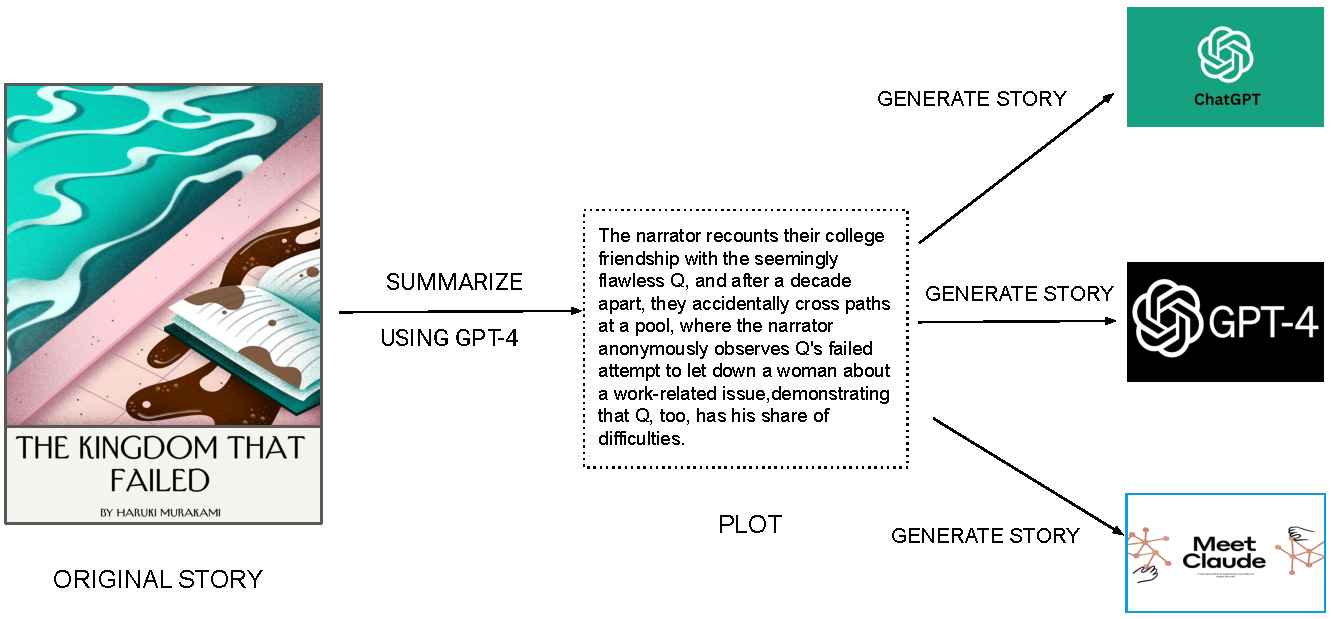
\includegraphics[width=\textwidth]{figures/datapipeline.pdf}
\caption{\label{datapipeline}Pipeline showing how our test set is created for evaluation. For each human-written original NewYorker story, we generate 3 stories from one LLM each, based on the plot of the original story. The plot is a single-sentence summary of the original story automatically generated by GPT-4 and verified by humans.}
\end{figure*}


In order to allow relative evaluation each human-authored narrative is summarized into a single-sentence plot, which is further verified by human evaluators. We then prompt three LLMs: GPT3.5, GPT4, and Claude, to generate a story conditioned on this plot summary. This yields a total of 48 short narratives for absolute evaluation (12 human written; 36 LLM written). Following this, we assign four stories centered around a single plot (one human-authored versus three LLM-authored) to a singular cluster, culminating in a total of 12 clusters. The methodology for creating an individual cluster is illustrated in Figure \ref{datapipeline}. The decision to employ human-authored plot summaries to prompt the LLMs is informed by the recognized shortfall of LLMs in their ability to devise original plotlines, as highlighted in previous research \cite{ippolito2022creative}. Furthermore, the utilization of multiple stories derived from the same plot enables experts to concentrate specifically on the human aspects of creative writing, and enhances their capacity to distinguish human-generated content from AI-produced ones.

In our quest to prevent straightforward parameters from differentiating between stories penned by human authors versus those produced by artificial intelligence (AI), we implemented strategies to ensure comparable story lengths across both classes. Initial experimentation revealed a notable discrepancy: Large Language Models (LLMs), when instructed to generate narratives of a predetermined word count, consistently underperformed, resulting in stories that were invariably more concise than intended. To address this inconsistency, we employed an iterative mechanism, prompting the LLM to iteratively rewrite the initial story until the divergence in word count between the AI-generated and human-composed story was less than 200 for every cluster. Table \ref{promptstory} (Row1) shows the original story prompt, while (Row2) illustrates the subsequent instruction to rewrite the story. We start the iterative process by prompting the LLM to expand the initially generated story. This cycle continued until the narrative length reached the pre-specified threshold or when the iteration count exceeded twenty ($loop\_count > $20). This methodology ensured the creation of AI-written stories with length characteristics more akin to those produced by human authors.

\begin{figure*}
\small
\centering
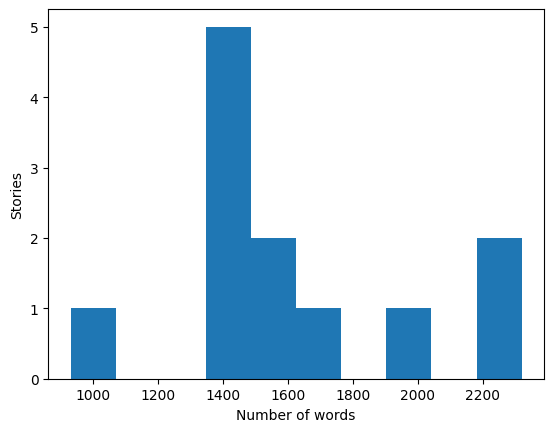
\includegraphics[width=\textwidth]{figures/length.png}
\caption{\label{length} Distribution of word count amongst the stories in our test set}
\end{figure*}


\begin{table}[]
\centering
\small
\def\arraystretch{1.35}
\begin{tabular}{|l|}
\hline
\begin{tabular}[c]{@{}l@{}}Write a New Yorker-style story given the plot below. Make sure it is atleast \textbf{\color{blue}\{\{word\_count\}\}} words. Directly start with the\\ story, do not say things like `Here's the story {[}...{]}:\end{tabular}                                                                                                                                                                                            \\ \hline\hline
\begin{tabular}[c]{@{}l@{}}You wrote the story I gave you below. I requested a story with \textbf{\color{blue}\{\{word\_count\}\}} words, but the story only has\\ \textbf{\color{blue}\{\{current\_word\_count\}\}} words. Can you rewrite the story to make it longer, and closer to the \textbf{\color{blue}\{\{word\_count\}\}} word target\\ I gave you. Directly start with the story, do not say things like `Here's the story {[}...{]}:`\\ \\ Current story: \{\{story\}\}\end{tabular} \\ \hline
\end{tabular}
\vspace{2ex}
\caption{\label{promptstory}Prompt to write the initial story (Row1) vs Prompt to rewrite the initial story to be longer. word\_count represents the number of words in the human written story on a given plot (P) while current\_word\_count represents the number of words in the LLM generated story on the same plot (P)}
\vspace{-7ex}
\end{table}

%     
%     \begin{subfigure}[b]{1.0\textwidth}
%          \centering
%          

\section{Model Architecture Design}
The overview of our \nameofmethod{} model is shown in Fig.~\ref{fig:hunyuanvideo_overview}. This section describes the Causal 3D VAE, diffusion backbone, and scaling laws experiments.

\label{sec:model_arch}
\begin{figure}[t]
    \centering
    \ifhq
    \includegraphics[trim={2cm 2cm 2cm 2cm},clip,width=0.95\linewidth]{hqfigures/hunyuanvideo_overview.pdf}
    \else
    \includegraphics[width=0.95\linewidth]{figures/hunyuanvideo_overview.png}
    \fi
    \caption{The overall architecture of \nameofmethod{}. The model is trained on a spatial-temporally compressed latent space, which is compressed through Causal 3D VAE. Text prompts are encoded using a large language model, and used as the condition. Gaussian noise and condition are taken as input, our model generates a output latent, which is decoded into images or videos through the 3D VAE decoder.}
    \label{fig:hunyuanvideo_overview}
\end{figure}

% \dq{add in architecture design of 3D VAE and DiT. Put diagram here also.}
\subsection{3D Variational Auto-encoder Design}\label{3dVAE}

Similar to previous work~\cite{polyak2024movie,yang2024cogvideox}, we train a 3DVAE to compress pixel-space videos and images into a compact latent space. To handle both videos and images, we adopt CausalConv3D~\cite{yu2023language}. For a video of shape $(T+1) \times 3 \times H \times W$, our 3DVAE compresses it into latent features with shape $(\frac{T}{c_t} + 1) \times C \times (\frac{H}{c_s}) \times (\frac{W}{c_s})$. In our implementation, $c_t=4$, $c_s=8$, and $C=16$. This compression significantly reduces the number of tokens for the subsequent diffusion transformer model, allowing us to train videos at the original resolution and frame rate. The model structure is illustrated in Figure \ref{fig:vae-model-arch}.

\begin{figure}[t]
    \centering
    \includegraphics[width=0.95\linewidth]{figures/vae-model-arch.pdf}
    \caption{ The architecture of our 3DVAE.}
    \label{fig:vae-model-arch}
\end{figure}

\subsubsection{Training}
In contrast to most previous work \cite{polyak2024movie,chen2024od,zhou2024allegro}, we do not rely on a pre-trained image VAE for parameter initialization; instead, we train our model from scratch. 
To balance the reconstruction quality of videos and images, we mix video and image data at a ratio of $4:1$. Besides the routinely used $L_1$ reconstruction loss and KL loss $L_{kl}$, we also incorporate perceptual loss $L_{lpips}$ and GAN adversarial loss $L_{adv}$ \cite{esser2021taming} to enhance the reconstruction quality. The complete loss function is shown in Equation \ref{eq:vae-loss}.

\begin{equation}
    \label{eq:vae-loss}
    \text{Loss} = L_{1} + 0.1 L_{lpips} + 0.05 L_{adv} + 10^{-6} L_{kl}
\end{equation}

During training, we employ a curriculum learning strategy, gradually training from low-resolution short video to high-resolution long video. To improve the reconstruction of high-motion videos, we randomly choose a sampling interval from the range $1 \sim 8$ to sample frames evenly across video clips.

\subsubsection{Inference}
Encoding and decoding high-resolution long videos on a single GPU can lead to out-of-memory (OOM) errors. To address this, we use a spatial-temporal tiling strategy, splitting the input video into overlapping tiles along the spatial and temporal dimensions. Each tile is encoded/decoded separately, and the outputs are stitched together. For the overlapping regions, we utilize a linear combination for blending. This tiling strategy allows us to encode/decode videos in arbitrary resolutions and durations on a single GPU.

We observed that directly using the tiling strategy during inference can result in visible artifacts due to inconsistencies between training and inference. To solve this, we introduce an additional finetuning phase where the tiling strategy is randomly enabled/disabled during training. This ensures the model is compatible with both tiling and non-tiling strategies, maintaining consistency between training and inference. 

\begin{figure}[ht]
    \centering
    \ifhq
    \includegraphics[width=\linewidth]{hqfigures/vae-sota-cmp.png}
    \else
    \includegraphics[width=\linewidth]{figures/vae-sota-cmp.pdf}
    \fi
    \caption{VAE reconstruction case comparison.}
    \label{fig:vae-sota-cmp}
\end{figure}

Table \ref{tab:sota_vae} compares our VAE with open-source state-of-the-art VAEs. On video data, our VAE demonstrates a significantly higher PSNR compared to other video VAEs. On images, our performance surpasses both video VAEs and image VAE. Figure \ref{fig:vae-sota-cmp} shows several cases at $256 \times 256$ resolution. Our VAE demonstrates significant advantages in text, small faces, and complex textures.
%Table \ref{tab:sota_vae} compares our VAE with open-source state-of-the-art VAEs. On video data, our VAE demonstrates a significantly higher PSNR compared to other video VAEs, achieving performance comparable to frame-wise image VAE while maintaining a 4x higher temporal compression. On images, our PSNR not only surpasses that of other video VAEs but also exceeds that of image VAE. Figure \ref{fig:vae-sota-cmp} shows several cases at $256 \times 256$ resolution. It is evident that our VAE demonstrates significant advantages in  text, small faces, and complex textures.


\begin{table*}[ht]
\renewcommand{\arraystretch}{1.2}
\small
\centering  
\caption{VAE reconstruction metrics comparison.}
\begin{tabular}{lcccc}
\toprule
\multirow{2}{*}{Model} & Downsample  & \multirow{2}{*}{$|z|$} & ImageNet (256$\times$256)
& MCL-JCV (33$\times$360$\times$640) \\
& Factor & & PSNR$\uparrow$ & PSNR$\uparrow$ \\
\midrule
%FLUX-VAE~\cite{FLUX}                   & $1 \times 8 \times 8$ & 16 & 32.70 & 37.87 \\
FLUX-VAE~\cite{FLUX}                   & $1 \times 8 \times 8$ & 16 & 32.70 & - \\
\midrule
OpenSora-1.2~\cite{opensora}           & $4 \times 8 \times 8$ & 4  & 28.11 & 30.15 \\
CogvideoX-1.5~\cite{yang2024cogvideox} & $4 \times 8 \times 8$ & 16 & 31.73 & 33.22 \\
Cosmos-VAE~\cite{cosmos}               & $4 \times 8 \times 8$ & 16 & 30.07 & 32.76 \\
Ours                                   & $4 \times 8 \times 8$ & 16 & 33.14 & 35.39 \\
\bottomrule
\end{tabular}
\label{tab:sota_vae}
\end{table*}

% \dq{@Common Utility Team}

\input{tax/scaling_law}

\input{tax/pre-training}

% \input{tax/t2v}

\input{tax/accelerate}



\section{Fundation Model Performance}
\label{sec:exp}

\myPara{Text Alignment}
% \dq{@Tianqi, Weijie, Daquan}
One of the key metrics for video generative models is their ability to follow text prompts accurately. This capability is essential for the effectiveness of these models. However, some open-source models often struggle to capture all subjects or accurately represent the relationships between multiple subjects, particularly when the input text prompt is complex.
%
\nameofmethod{} demonstrates robust capabilities in generating videos that closely adhere to the provided text prompts. As illustrated in Figure \ref{fig:text-align}, it effectively manages multiple subjects within the scene.

\begin{figure}[h]
    \centering
    \ifhq
    \includegraphics[trim={0cm 5cm 0cm 4cm},clip,width=\linewidth]{hqfigures/text_alignment.pdf}
    \else
    \includegraphics[width=\linewidth]{figures/text_alignment.png}
    \fi
    \caption{{Prompt: A white cat sits on a white soft sofa like a person, while its long-haired male owner, with his hair tied up in a topknot, sits on the floor, gazing into the cat's eyes. His child stands nearby, observing the interaction between the cat and the man. } }
    \label{fig:text-align}
\end{figure}


\myPara{High-quality}
% \dq{@Jodai}
We also perform a fine-tuning process to enhance the spatial quality of the generated videos. As illustrated in Figure \ref{fig:high_quality}, \nameofmethod{} is capable of producing videos with ultra-detailed content.
\begin{figure}[!htbp]
    \centering
    \begin{subfigure}{\textwidth}
        \centering
        \ifhq
        \includegraphics[width=\textwidth]{hqfigures/high-quality-1.pdf}
        \else
        \includegraphics[width=\textwidth]{figures/high-quality-1.png}
        \fi
        \caption{Prompt: the ultra-wide-angle lens follows closely from the hood, with raindrops continuously splattering against the lens. Ahead, a sports car speeds around a corner, its tires violently skidding against the wet road, creating a mist of water. Neon lights refract in the rain, leaving colorful streaks on the car's surface. The camera swiftly shifts to the side of the car, capturing the wheels spinning at high speed, before finally moving to the rear.}
    \end{subfigure}
    \hfill
    \begin{subfigure}{\textwidth}
        \centering
        \ifhq
        \includegraphics[width=\textwidth]{hqfigures/high-quality-2.pdf}
        \else
        \includegraphics[width=\textwidth]{figures/high-quality-2.png}
        \fi
        \caption{Prompt: a stylish woman walks down a Tokyo street filled with warm glowing neon and animated city signage. She wears a black leather jacket, a long red dress, and black boots, and carries a black purse. She wears sunglasses and red lipstick. She walks confidently and casually. The street is damp and reflective, creating a mirror effect of the colorful lights. Many pedestrians walk about.}
    \end{subfigure}
    \caption{High-quality videos generated by HunyuanVideo.}
    \label{fig:high_quality}
\end{figure}

\myPara{High-motion Dynamics}
% \dq{@Weijie, Junkun}
In this part, we demonstrate \nameofmethod{}'s capabilities in producing high-dynamic videos based on given prompts. As shown in Figure \ref{fig:high_motion}, our model excels in generating videos that encompass a wide range of scenes and various types of motion.

\begin{figure}[!htbp]
    \centering
    \begin{subfigure}{\textwidth}
        \centering
        \ifhq
        \includegraphics[trim={4.8cm 4.8cm 4.8cm 4.8cm},clip,width=0.95\textwidth]{hqfigures/high_motion_3.pdf}
        \else
        \includegraphics[width=\textwidth]{figures/high_motion_3.jpg}
        \fi
        \captionsetup{font=small}
        \caption{Prompt: At sunset, a modified Ford F-150 Raptor roared past on the off-road track. The raised suspension allowed the huge explosion-proof tires to flip freely on the mud, and the mud splashed on the roll cage.}
        \label{fig:hm_1}
    \end{subfigure}
    \hfill
    \begin{subfigure}{\textwidth}
        \centering
        \ifhq
        \includegraphics[trim={4.8cm 4.8cm 4.8cm 4.8cm},clip,width=0.95\textwidth]{hqfigures/high_motion_5.pdf}
        \else
        \includegraphics[width=\textwidth]{figures/high_motion_5.jpg}
        \fi
        \captionsetup{font=small}
        \caption{Prompt: The panning camera moves forward slowly, with a depth of field in the middle focus, and warm sunset light covers the screen. The girl in the picture runs with her skirt fluttering, turns and jumps.}
        \label{fig:hm_2}
    \end{subfigure}
    \hfill
    \begin{subfigure}{\textwidth}
        \centering
        \ifhq
        \includegraphics[trim={4.8cm 4.8cm 4.8cm 4.8cm},clip,width=0.95\textwidth]{hqfigures/high_motion_2.pdf}
        \else
        \includegraphics[width=\textwidth]{figures/high_motion_2.jpg}
        \fi
        \captionsetup{font=small}
        \caption{Prompt: In the gym, a woman in workout clothes runs on a treadmill. Side angle. Realistic, Indoor lighting, Professional.}
        \label{fig:hm_3}
    \end{subfigure}
    \hfill
    \begin{subfigure}{\textwidth}
        \centering
        \ifhq
        \includegraphics[trim={4.8cm 4.8cm 4.8cm 4.8cm},clip,width=0.95\textwidth]{hqfigures/high_motion_7.pdf}
        \else
        \includegraphics[width=\textwidth]{figures/high_motion_7.jpg}
        \fi
        \captionsetup{font=small}
        \caption{Prompt: Swimmer swimming underwater, in slow motion. Realistic, Underwater lighting, Peaceful.}
        \label{fig:hm_4}
    \end{subfigure}
    \hfill
    \begin{subfigure}{\textwidth}
        \centering
        \ifhq
        \includegraphics[trim={4.8cm 4.8cm 4.8cm 4.8cm},clip,width=0.95\textwidth]{hqfigures/high_motion_8.pdf}
        \else
        \includegraphics[width=\textwidth]{figures/high_motion_8.jpg}
        \fi
        \captionsetup{font=small}
        \caption{Prompt: On the rooftop, there is an open-air basketball court, and five male students are playing basketball. Realistic, Natural lighting, Casual.}
        \label{fig:hm_5}
    \end{subfigure}
    \caption{High-motion dynamics videos generated by \nameofmethod{}.}
    \label{fig:high_motion}
\end{figure}


\myPara{Concept Generalization}
% \dq{@Daquan, Zhiyu}
One of the most desirable features of a generative model is its ability to generalize concepts. As illustrated in Figure \ref{fig:concept}, the text prompt describes a scene: "In a distant galaxy, an astronaut floats on a shimmering, pink, gemstone-like lake that reflects the vibrant colors of the surrounding sky, creating a stunning scene. The astronaut gently drifts on the lake's surface, while the soft sounds of water whisper the planet's secrets. He reaches out, his fingertips gliding over the cool, smooth water." Notably, this specific scenario has not been encountered in the training dataset. Furthermore, it is evident that the depicted scene combines several concepts that are also absent from the training data.
\begin{figure}[!htbp]
    \centering
    \ifhq
    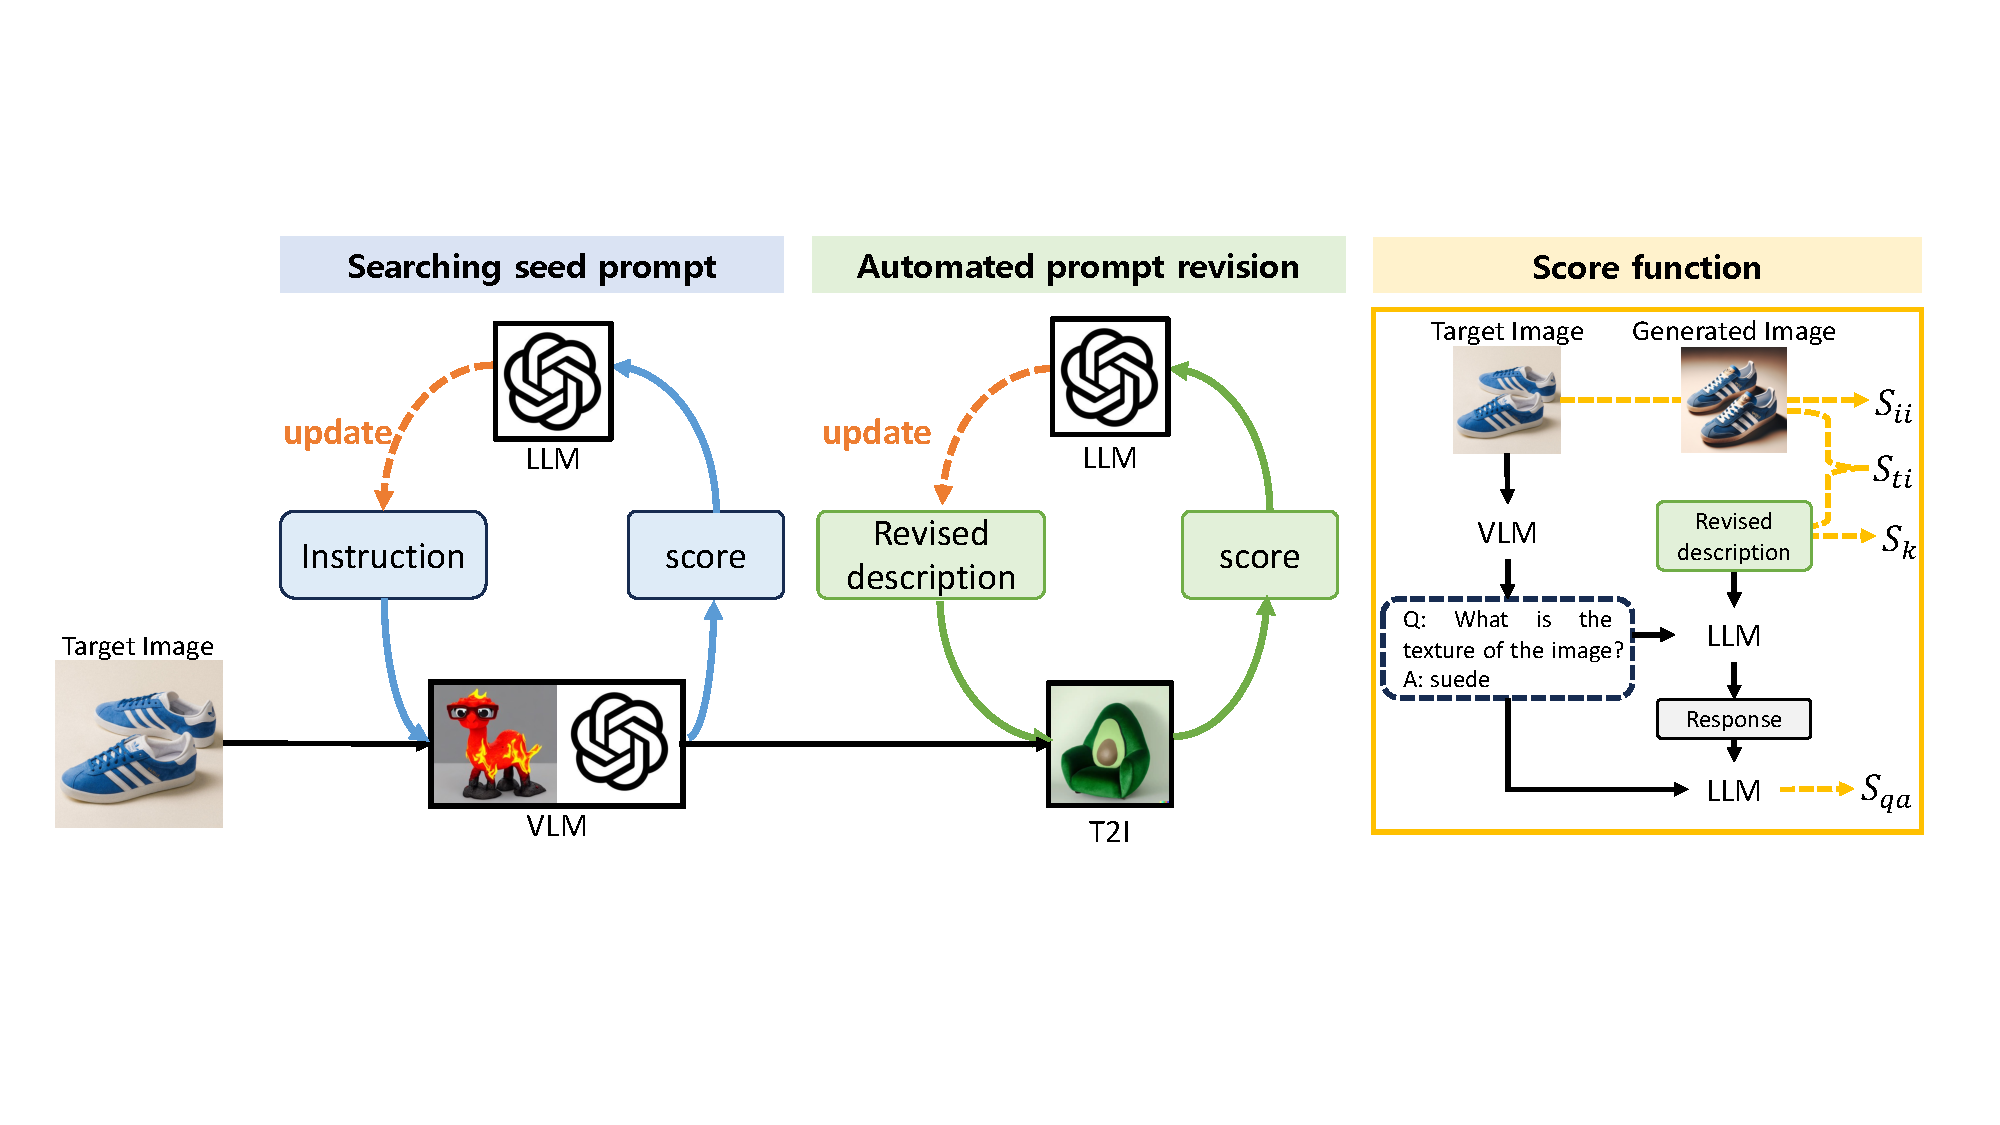
\includegraphics[trim=0cm 5cm 0cm 4cm,clip,width=\linewidth]{hqfigures/concept.pdf}
    \else
    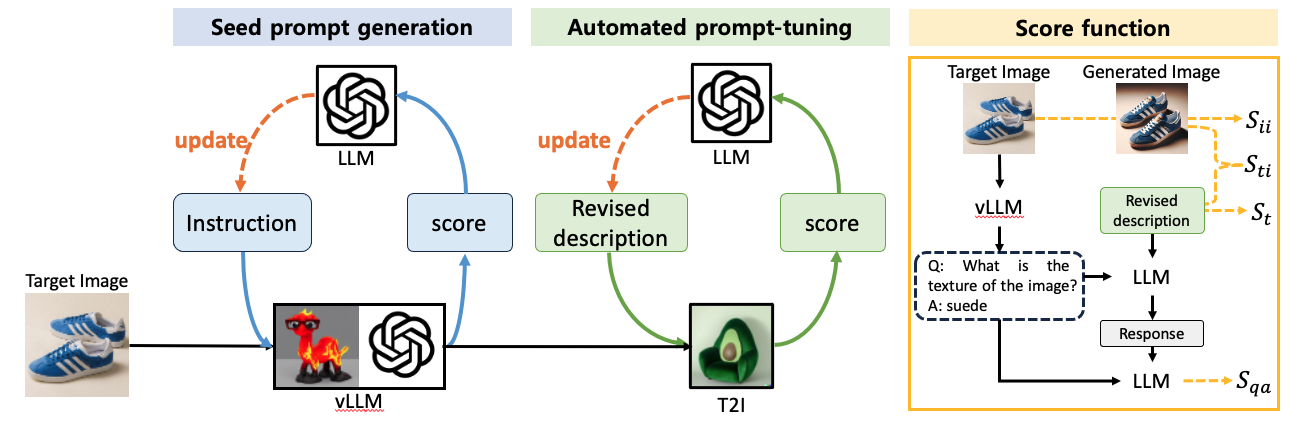
\includegraphics[width=\linewidth]{figures/concept.png}
    \fi
    \caption{\small {\nameofmethod{}'s performance on concept generalization. The results of the three rows correspond to the text prompts (1) `In a distant galaxy, an astronaut floats on a shimmering, pink, gemstone-like lake that reflects the vibrant colors of the surrounding sky, creating a stunning scene. The astronaut gently drifts on the lake's surface, the soft sounds of water whispering the planet's secrets. He reaches out, his fingertips gliding over the cool, smooth water. ', (2) `A macro lens captures a tiny orchestra of insects playing instruments.' and (3) `The night-blooming cactus flowers in the evening, with a brief, rapid closure. Time-lapse shot, extreme close-up. Realistic, Night lighting, Mysterious.' respectively.} }
    \label{fig:concept}
\end{figure}

\myPara{Action Reasoning and Planning}
% \dq{@Li Xin}
Leveraging the capabilities of large language models, \nameofmethod{} can generate sequential movements based on a provided text prompt. As demonstrated in Figure \ref{fig:sequential-move}, \nameofmethod{} effectively captures all actions in a photorealistic style.
\begin{figure}[ht]
    \centering
    \ifhq
    \includegraphics[trim=0cm 5cm 0cm 4cm,clip,width=\linewidth]{hqfigures/sequential_motion.pdf}
    \else
    \includegraphics[width=\linewidth]{figures/sequential_motion.png}
    \fi
    \caption{{Prompt: The woman walks over and opens the red wooden door. As the door swings open, seawater bursts forth, in a realistic style.}}
    \label{fig:sequential-move}
\end{figure}

\myPara{Character Understanding and Writing}
\nameofmethod{} is capable of generating both scene text and gradually appearing handwritten text as shown in Fig.~\ref{fig:ocr}. 



% \dq{@Wuyue}
\begin{figure}[!htbp]
    \centering
    \ifhq
    \includegraphics[trim=2cm 5cm 2cm 4cm,clip,width=\linewidth]{hqfigures/ocr.pdf}
    \else
    \includegraphics[width=\linewidth]{figures/ocr.png}
    \fi
    \caption{High text-video alignment videos generated by HunyuanVideo. Top row: Prompt: A close-up of a wave crashing against the beach, the sea foam spells out ``WAKE UP'' on the sand. Bottom row: Prompt: In a garden filled with blooming flowers, ``GROW LOVE'' has been spelled out with colorful petals.}
    \label{fig:ocr}
\end{figure}





\input{exp/human_eval}

\section{Applications}
\label{sec:application}

\subsection{Audio Generation based on Video}
% \dq{@yutao, james, miles}

Our video-to-audio(V2A) module is designed to enhance generated video content by incorporating synchronized sound effects and contextually appropriate background music. Within the conventional film production pipeline, Foley sound design constitutes an integral component, significantly contributing to the auditory realism and emotional depth of visual media. However, the creation of Foley audio is both time-intensive and demands a high degree of professional expertise. With the advent of an increasing number of text-to-video (T2V) models, most of them lack the corresponding foley generation capabilities, thereby limiting their ability to produce fully immersive content. Our V2A module addresses this critical gap by autonomously generating cinematic-grade foley audio tailored to the input video and textual prompts, thus enabling the synthesis of a cohesive and holistically engaging multimedia experience.

\subsubsection{Data }
Unlike text-to-video (T2V) models, video-to-audio (V2A) models have different requirements for data. As mentioned above, we constructed a video dataset comprising of video-text pairs. However, not all data in this dataset are suitable for training the V2A model. For example, some videos lack an audio stream, others contain extensive voice-over content or their ambient audio tracks have been removed and replaced with unrelated elements. To address these challenges and ensure data quality, we designed a robust data filtering pipeline specifically tailored for V2A training.

First, we filter out videos without audio streams or those in which the silence ratio exceeds 80\%. Next, we employ a frame-level audio detection model, like \cite{Hung2022}, to detect speech, music, and general sound in the audio stream. Based on this analysis, we classify the data into four distinct categories: \textit{pure sound}, \textit{sound with speech}, \textit{sound with music}, and \textit{pure music}. Subsequently, to prioritize high-quality data, we train a model inspired by CAVP \cite{luo2024diff} to compute a visual-audio consistency score, which quantifies the alignment between the visual and auditory components of each video. Using this scoring system in conjunction with the audio category labels, we systematically sample portions of data from each category, retaining approximately 250,000 hours from the original dataset for pre-training. For the supervised fine-tuning stage, we further refine our selection, curating a subset of millions of high-quality clips~(80,000 hours).

For feature extraction, we use CLIP \cite{clip} to obtain visual features at a temporal resolution of 4 fps and subsequently resample these features to align with the audio frame rate. To generate captions, we employ \cite{haji2024taming} as the sound captioning model and \cite{doh2023lp} as the music captioning model. When both sound and music captions are available, we merge them into a structured caption format, following the approach detailed in \cite{polyak2024movie}.


\begin{figure}[t]
    \centering
    \ifhq
    \includegraphics[trim={5cm 5cm 5cm 5cm},clip,width=0.9\linewidth]{hqfigures/vt2a_arch.pdf}
    \else
    \includegraphics[width=0.9\linewidth]{figures/vt2a_arch.png}
    \fi
    \caption{The architecture of sound effect and music generation model. }
    \label{fig:audio-gen}
\end{figure}

\subsubsection{Model}
Just like the above-mentioned text-to-video model, our video-to-audio generation model also adopts a flow-matching-based diffusion transformer (DiT) as its architectural backbone. The detailed design of the model is depicted in Figure \ref{fig:audio-gen}, illustrating a transition from a triple-stream structure to a single-stream DiT framework.

The model operates within a latent space encoded by a variational autoencoder (VAE) trained on mel-spectrograms. Specifically, the audio waveform is first converted into a 2D mel-spectrogram representation. This spectrogram is subsequently encoded into a latent space using a pretrained VAE. For feature extraction, we leverage pretrained CLIP \cite{clip} and T5 \cite{raffel2020exploring} encoders to independently extract visual and textual features, respectively. These features are subsequently projected into the DiT-compatible latent space using independent linear projections followed by SwiGLU activation, as depicted in Figure \ref{fig:audio-gen}.

To effectively integrate multimodal information, we incorporate stacked triple-stream transformer blocks, which independently process visual, audio, and textual modalities. These are later followed by single-stream transformer blocks to ensure seamless fusion and alignment across modalities. This design enhances the alignment between audio-video and audio-text representations, facilitating improved multimodal coherence.

Once the latent representation is generated by the diffusion transformer, the VAE decoder reconstructs the corresponding mel-spectrogram. Finally, the mel-spectrogram is converted back into an audio waveform using a pre-trained HifiGAN vocoder \cite{kong2020hifi}. This framework ensures a high-fidelity reconstruction of audio signals while maintaining strong multimodal alignment.



\subsection{Hunyuan Image-to-Video}
% \dq{Tianqi, Weijie, Daquan}
\subsubsection{Pre-training}
\begin{figure}[t]
    \centering
    \ifhq
    \includegraphics[trim={5cm 5cm 5cm 5cm},clip,width=0.9\linewidth]{hqfigures/I2V.pdf}
    \else
    \includegraphics[width=0.9\linewidth]{figures/I2V.pdf}
    \fi
    \caption{Differences between text-to-video (T2V) model and image-to-video (I2V) model.}
    \label{fig:i2v}
\end{figure}
Image-to-video (I2V) task is a common application in video generation tasks. It usually means that given an image and a caption, the model uses this image as the first frame to generate a video that matches the caption.
Although the naive \nameofmethod{} is a text-to-video (T2V) model, it can be easily extended to an I2V model.
Specifically, as mentioned in Sec. \ref{sec:architecture}, the T2V model's input is a latent $X$ with a shape of $T \times C \times H \times W$, where $T$, $C$, $H$ and $W$ represent the frame, channel, height and width of the compressed video respectively.
Similar to Emu \cite{girdhar2023emu}, in order to introduce image condition $I$, we treat $I$ as the first frame of a video and apply zero-padding to create a $T \times C \times H \times W$ tensor $I_o$, as shown in Fig. \ref{fig:i2v}.
Additionally, we employ a binary mask $m$ with dimensions $T \times 1 \times H \times W$, where the first temporal position is set to 1, and all other positions are set to zero. Then the latent $X$, the tensor $I_o$ and the mask $m$ are concatenated along the channel dimension to form the input for the model.
Note that since the channel of the input tensor has changed from $C$ to $2C+1$, as shown in Fig. \ref{fig:i2v}, we need to adjust the parameters of the first convolutional module of the model from $\phi=(C_{in}(=C), C_{out}, s_h, s_w)$ to $\phi^{\prime}=(C_{in}^{\prime}(=2C+1), C_{out}, s_h, s_w)$, where each component corresponds to the input channel $C_{in}/C_{in}^{\prime}$, output channel $C_{out}$, height of the convolutional kernel $s_h$, and width of the convolutional kernel $s_w$.
In order to retain the representation ability of the T2V model, the first $C$ input channels of $\phi^{\prime}$ are directly copied to $\phi$, and the rest are initialized to zero. We pre-train the I2V model on the same data as T2V model, and the results are shown in Fig. \ref{fig:i2v_result}.
\begin{figure}[t]
    \centering
    \ifhq
    \includegraphics[width=\linewidth]{hqfigures/i2v_pretraining_result.png}
    \else
    \includegraphics[width=\linewidth]{figures/i2v_pretraining_result.png}
    \fi
    \caption{Sample results of the I2V pre-training model.}
    \label{fig:i2v_result}
\end{figure}


\subsubsection{Downstream Task Fine-tuning: Portrait Image-to-Video Generation}
We perform supervised finetuning of our I2V model on two million portrait videos to enhance human's motion and overall aesthetics. In addition to the standard data filtering pipeline described in section \ref{sec:data}, we also apply face and body detectors to filter out the training videos which have more than five persons. We also remove the videos in which the main subjects are small. Finally, the rest videos will be manually inspected to obtain the final high-quality portrait training dataset.

Regarding training, we adopt a progressive fine-tuning strategy, gradually unfreezing the model parameters of the respective layers while keeping the rest frozen during finetuning. This approach allows the model to achieves high performance in the portrait domain without compromising much of its inherent generalization ability, guaranteeing commendable performance in natural landscapes, animals, and plants domains. Moreover, our model also supports video interpolation by using the first and last frames as conditions. We randomly drop the text conditions at certain probability during training to enhance the model's performance. Some demo results are shown in Fig. \ref{fig:portrait_i2v}.

\begin{figure}[h]
    \centering
    \includegraphics[width=\linewidth]{applications/app_figures/portrait_to_video_new.png}
    \caption{Sample results of our portrait I2V model.}
    \label{fig:portrait_i2v}
\end{figure}

\subsection{Avatar animation}
% \dq{Application Center}

{\nameofmethod} empowers controllable avatar animation in various aspects. It enables animating characters using explicit driving signals(e.g., speech signals, expression templates, and pose templates). In addition, it also integrates the implicit driving paradigm using text prompts. Fig. \ref{fig:application-method} shows how we leverage the power of {\nameofmethod} to animate characters from multi-modal conditions. To maintain strict appearance consistency, we modify the {\nameofmethod} architecture by inserting latent of reference image as strong guidance. As shown in Fig. \ref{fig:application-method} (b, c), we encode reference image using 3DVAE obaining $z_{\rm ref} \in \mathbb{R}^{1 \times c \times h \times w}$, where $c = 16$. Then we repeat it $t$ times along temporal dimension and concatenate with $z_t$ in channel dimension to get the modified noise input $\hat{z}_t \in \mathbb{R}^{t \times 2c \times h \times w}$. To achieve controllable animation, various adapters are employed. We describe them in following.

\begin{figure}[h]
    \centering
    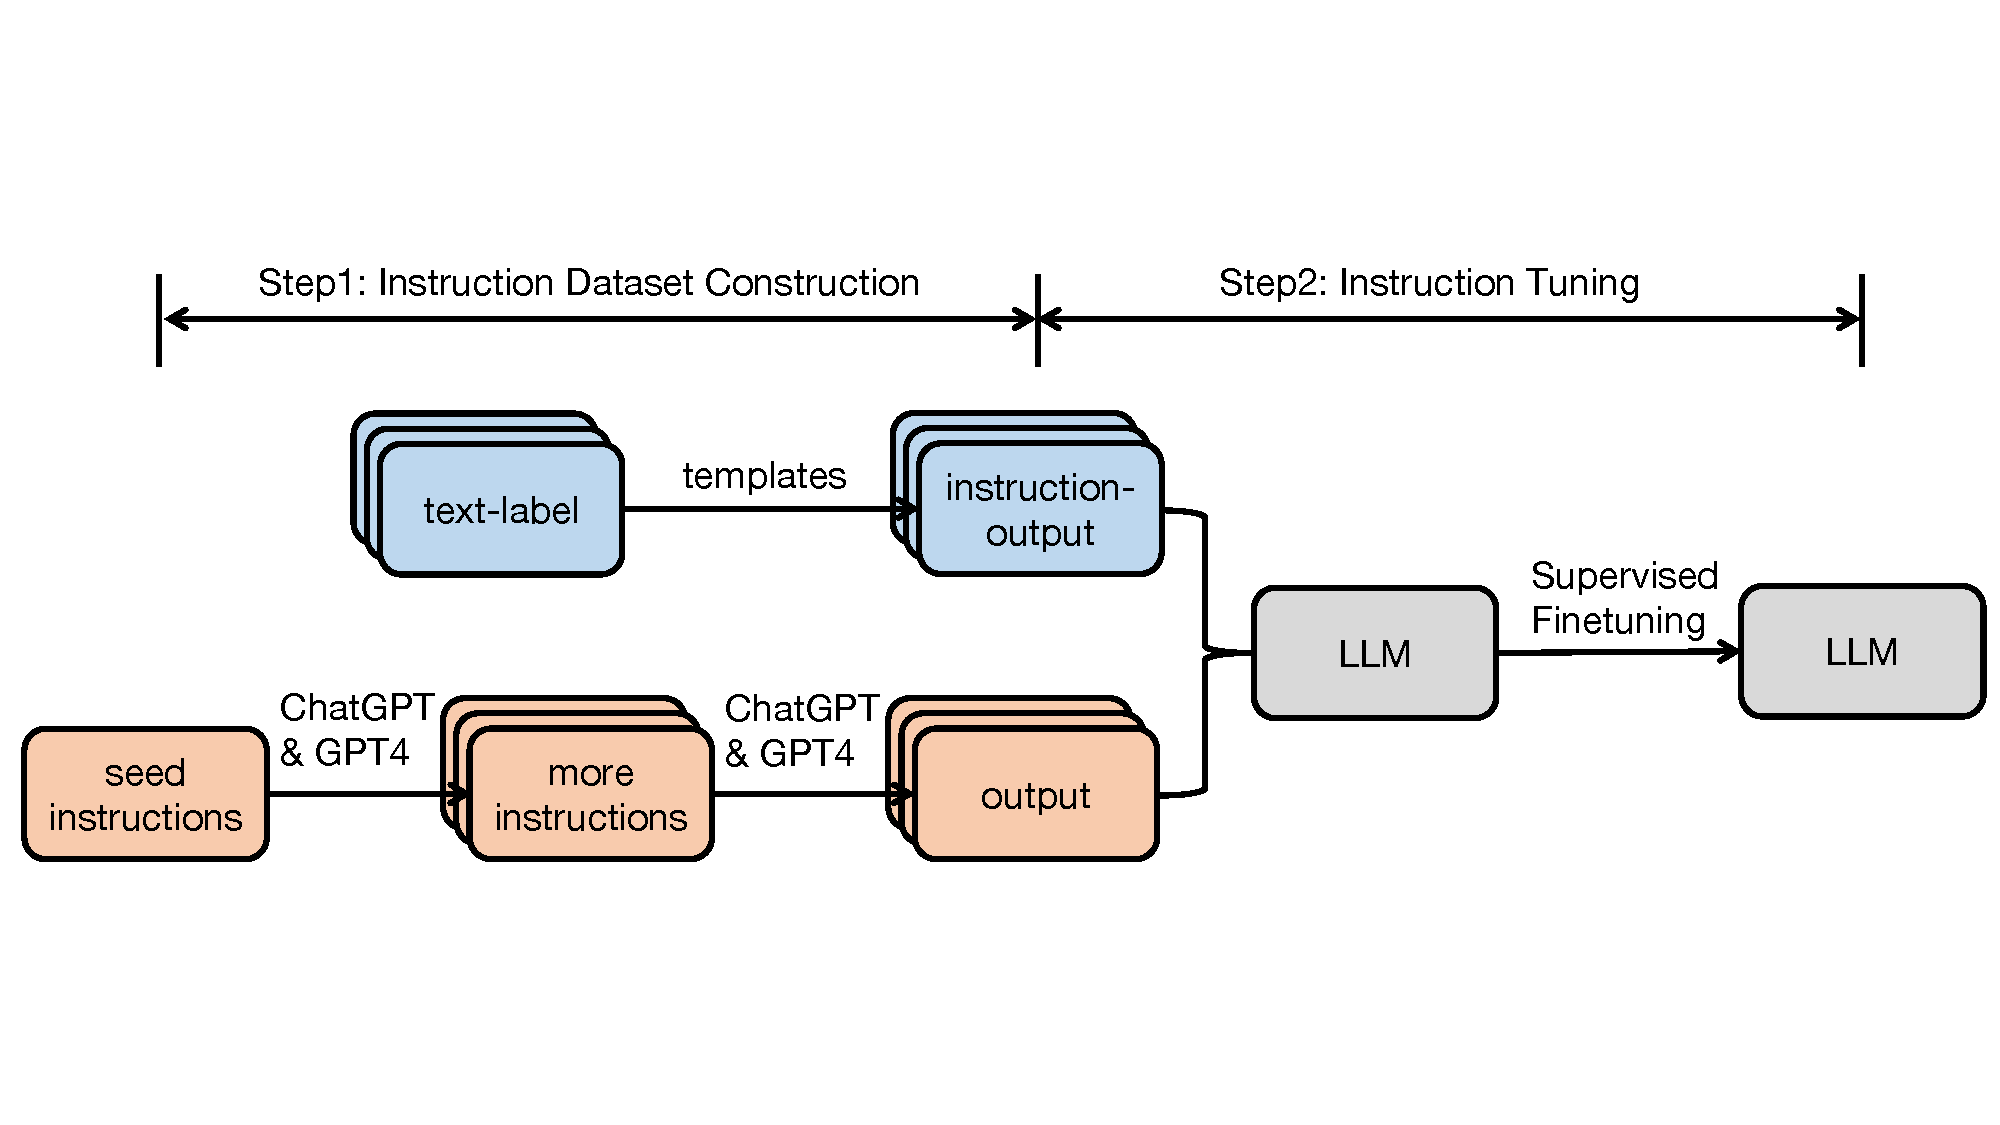
\includegraphics[width=\linewidth]{applications/app_figures/method.pdf}
    \caption{\textbf{Overview of Avatar Animation built on top of \nameofmethod}. We adopt 3D VAE to encode and inject reference and pose condition, and use additional cross-attention layers to inject audio and expression signals. Masks are employed to explicitly guide where they are affecting.}
    \label{fig:application-method}
\end{figure}

\subsubsection{Upper-Body Talking Avatar Generation}

In recent years, audio-driven digital human algorithms have made significant progress, especially in the performance of the talking head. Early algorithms, such as loopy~\cite{ye2024mimic}, emo~\cite{tian2024emo}, and hallo~\cite{xu2024hallo}, mainly focused on the head area, driving the digital human's facial expressions and lip shapes by analyzing audio signals. Even earlier algorithms, like wav2lip~\cite{prajwal2020lip} and DINet~\cite{zhang2023dinet}, concentrated on modifying the mouth region in the input video to achieve lip shape consistency with the audio. However, these algorithms are usually limited to the head area, neglecting other parts of the body. To achieve a more natural and vivid digital human performance, we propose an audio-driven algorithm extended to the upper body. In this algorithm, the digital human not only synchronizes facial expressions and lip shapes with the audio while speaking but also moves the body rhythmically with the audio.

% \subsubsection{Audio-Driven}
\paragraph{Audio-Driven}
Based on the input audio signal, our model can adaptively predict the digital human's facial expressions and posture action information . This allows the driven character to speak with emotion and expression, enhancing the digital human's expressiveness and realism. 
As shown in  Fig. \ref{fig:application-method} (b), for the single audio signal-driven part, the audio passes through the whisper feature extraction module to obtain audio features, which are then injected into the main network in a cross-attention manner. It should be noted that the injection process will be multiplied by the face-mask to control the audio's effect area. While enhancing the head and shoulder control ability, it will also greatly reduce the probability of body deformation. To obtain more lively head movements, head pose motion parameters and expression motion parameters are introduced and added to the time step in an embedding manner. During training, the head motion parameters are given by the variance of the nose tip keypoint sequence, and the expression parameters are given by the variance of the facial keypoints. 
% During inference, fixed values pose=8 and exp=16 are used for inference.
% However, since there is no strong semantic correlation between audio itself and gestures, for some scenes, single audio-driven may cause the head and shoulder part to move naturally with the audio, but the body part, especially the hands,  tends to move slightly or unnaturally. To solve this problem, we introduce text information.


% \subsubsection{Audio and Text Driven}
% \paragraph{Audio and Text Driven}
% Based on aries' powerful semantic understanding ability, we inject a prompt describing actions as the model's text information. In this way, during video generation, the model can not only use audio signals to drive the digital human's actions but also refer to text information to provide more accurate and natural action information. 

% Unlike audio-driven, when we jointly drive with audio and text, we remove the face-mask, allowing the audio's effect area to be released and enabling the character to have a larger range of motion. Second, we removed the encoding of reference images based on llava. During audio-driven, without text injection, we use reference images for information injection. When there is text information, we prioritize aligning with the model's original input. Additionally, we retain the head pose motion parameters and expression parameters.

% By combining audio and text information, our algorithm can achieve a more natural and lively digital human performance. This method not only improves the realism of the digital human but also enhances its adaptability and expressiveness in different scenarios. 


\begin{figure}
    \centering
    \ifhq
    
\includegraphics[width=\linewidth]{hqapplications/audio.png}
    \else
    \includegraphics[width=\linewidth]{applications/app_figures/audio-1.pdf}
    \fi
    \caption{\textbf{Audio-Driven}. {\nameofmethod} can generate vivid talking avatar videos.}
    \label{fig:application-audio}
\end{figure}

\begin{figure}
    \centering
    \ifhq
    \includegraphics[width=\linewidth]{hqapplications/pose.png}
    \else
    \includegraphics[width=\linewidth]{applications/app_figures/pose.pdf}
    \fi
    \caption{\textbf{Pose-Driven}. {\nameofmethod} can animate wide variety of characters with high quality and appearance consistency under various poses.}
    \label{fig:application-pose}
\end{figure}


\begin{figure}
    \centering
    \ifhq
    \includegraphics[width=\linewidth]{hqapplications/expr.png}
    \else
    \includegraphics[width=\linewidth]{applications/app_figures/expr-1.pdf}
    \fi
    \caption{\textbf{Expression-Driven}. {\nameofmethod} can accurately control facial movements of wide-variety of avatar styles.}
    \label{fig:application-expr}
\end{figure}

\begin{figure}[h]
    \centering
    \ifhq
    \includegraphics[width=\linewidth]{hqapplications/pose-expr.png}
    \else
    \includegraphics[width=\linewidth]{applications/app_figures/pose-expr-1.pdf}
    \fi
    \caption{\textbf{Hybrid Condition-Driven}. {\nameofmethod} supports full control with multiple driving sources across various avatar characters.}
    \label{fig:application-pose-expr}
\end{figure}

\input{applications/expr_pose}

\input{applications/demo}


\section{Related Works}
\label{sec:related_works}

Due to the success of diffusion models in the field of image generation~\citep{rombach2022high, ho2020denoising}, the exploration in the domain of video generation~\citep{guo2023animatediff,jiang2023text2performer,singer2022make,wang2023lavie,yang2023probabilistic,zhang2023show,ma2024follow,chen2024follow,xue2024follow,ma2024follow2} is also becoming popular. VDM~\citep{ho2022video} is among the first that extends the 2D U-Net from image diffusion models to a 3D U-Net to achieve text-based generation.
%
Later works, such as MagicVideo~\citep{zhou2023magicvideo} and Mindscope~\citep{wang2023modelscope}, introduce 1D temporal attention mechanisms, reducing computations by building upon latent diffusion models. In this report, we do not use the 2D + 1D temporal block manner for motion learning. Instead, we use similar dual flow attention blocks as in FLUX \cite{FLUX}, which are used for processing all video frames.
%
Following Imagen, Imagen Video~\citep{ho2022imagen} employs a cascaded sampling pipeline that generates videos through multiple stages.
%
In addition to traditional end-to-end text-to-video (T2V) generation, 
video generation using other conditions is also an important direction.
%
This type of methods generates videos with other auxiliary controls, such as depth maps~\citep{guo2023sparsectrl,he2023animate}, pose maps~\citep{xu2023magicanimate,hu2023animate,wang2023disco,ma2023follow}, RGB images~\citep{blattmann2023stable,chen2023seine,ni2023conditional}, or other guided motion videos~\citep{zhao2023motiondirector,wu2023lamp}.  
%
Despite the excellent generation performance of the recent open-source models such as Stable video diffusion~\citep{blattmann2023stable}, Open-sora \cite{opensora}, Open-sora-plan \cite{pku_yuan_lab_and_tuzhan_ai_etc_2024_10948109}, Mochi-1 \cite{genmo2024mochi} and Allegro \cite{zhou2024allegro}, their performance still falls far behind the closed-source
%
state-of-the-art video generation models such as Sora \cite{videoworldsimulators2024} and MovieGen \cite{polyak2024movie}. 


\input{tax/contributors}

\clearpage
{%\small
\bibliographystyle{plain}
\bibliography{egbib}
}

\end{document}